\chapter{Fundamentação Teórica}
\label{chap:fundteor}

\begin{flushright}

   \begin{list}{}{
      \setlength{\leftmargin}{4.5cm}
      \setlength{\rightmargin}{0cm}
      \setlength{\labelwidth}{0pt}
      \setlength{\labelsep}{\leftmargin}}
      \item Quanto maior for a rapidez de transformação de uma
      sociedade, mais temporárias são as necessidades
      individuais. Essas flutuaçõess tornam ainda mais acelerado
      o senso de turbilh da sociedade.

      \begin{list}{}{
      \setlength{\leftmargin}{0cm}
      \setlength{\rightmargin}{0cm}
      \setlength{\labelwidth}{0pt}
      \setlength{\labelsep}{\leftmargin}}
      \item (Alvin Toffler)
      \end{list}
   \end{list}
\end{flushright}

\begin{flushright}
  Quanto maior for a rapidez de transformação de uma \\
  sociedade, mais temporárias são as necessidades \\
  individuais. Essas flutuações tornam ainda mais \\
  acelerado o senso de turbilhão da sociedade. \\
  \ \\
  (Alvin Toffler)
\end{flushright}

%--------- NEW SECTION ----------------------
\section{Micromouse}
\label{sec:Micromouse}
\hspace{0.5cm} A competição Micromouse é um concurso anual na qual estudantes do mundo todo desenvolvem pequenos robôs autônomos, chamados \textit{micromouse}, postos a correr dentro de um labirinto. Dessa forma, o \textit{micromouse} que mais rápido chegar ao seu centro é o vencedor da competição.

\begin{figure}[H]
	\centering
	\caption{Moonlight Special - Primeiro modelo \textit{micromouse} a ganhar uma competição.}
	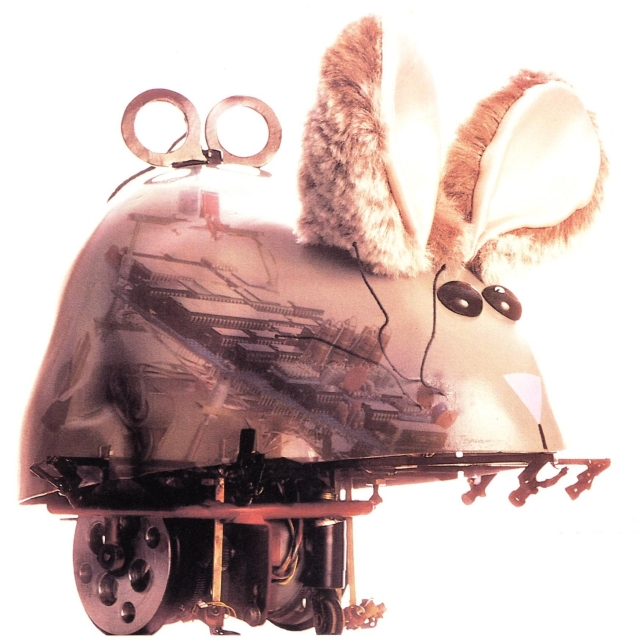
\includegraphics[width=0.6\textwidth]
	{Figures/MoonlightSpecial.jpg}
	\label{fig:MoonlightSpecial}
	\newline
	\source{FONTE}
\end{figure}

\hspace{0.5cm} Sua ideia surge em 1977, quando a \textit{IEEE Spectrum Magazine} trouxe pela primeira vez o conceito de robôs autônomos para resolução de labirintos. Pouco tempo depois, sua primeira competição foi realizada, em junho de 1979, na primeira \textit{IEEE Amazing Micromouse Maze Contest} organizada na cidade de Nova York. Rapidamente, o conceito da competição se espalhou e, já no começo da década de 90, vários clubes voltados para Micromouse surgiam em escolas e universidades do mundo todo \cite{Tondr2004}.

\hspace{0.5cm} Atualmente, a \textit{IEEE Micromouse Competition} adota uma configuração que consiste em um labirinto de 16 x 16 blocos. Cada bloco possui 18 x 18 cm. As paredes, que possuem 5 cm de altura, são pintadas de branco de modo a ser reflexiva à luz infravermelha. O chão, por outro lado, é pintado de preto, para que não seja reflexivo. Além disso, os competidores sabem previamente que o \textit{micromouse} tem seu ponto de partida localizado em um dos cantos do labirintos, devendo alcançar o seu centro para terminar o desafio. Com base nisso, os participantes devem usar de algorítimos de busca para explorar o labirinto e encontrar a rota mais otimizada para o ponto de chegada estabelecido pela competição. O robô por sua vez, não pode ter suas dimensões maiores que uma seção de 25 x 25 cm. As regras completas estão dispostas como anexo no final do documento.

%--------- NEW SECTION ----------------------
\section{Robotics Frameworks}
\label{sec:robotic_frameworks}
A palavra robô foi utilizada pela primeira vez em 1921 em uma peça teatral pelo dramaturgo checoslovaco Karel Capek. A origem vem da palavra checa robota que significa “trabalho forçado” e tornou-se popular através de filmes como Metrópolis (1926). O dia em que a terra parou (1951) e Planeta proibido (1956). Apesar da inserção do termo robô ser datada de 1921, registros históricos da antiga civilização grega já propunha o desenvolvimento dos primeiros modelos de robôs. Esses tinham aspecto visual semelhante ao de um humano e ou animal, e utilizavam sistemas de pesos e bombas pneumáticas, porém não tinham nenhuma funcionalidade prática, social, e como a época ainda não existia sistemas de produção complexos, esse robôs também não tinham função voltada à produtividade. Era um mecanismo de simples movimentação e sem nenhuma finalidade real. Algum tempo depois, cientistas árabes se dedicaram em fomentar a idéia e pesquisar sobre atribuir possíveis funções a esses robôs, com objetivo de facilitar as necessidades humanas. Esse pensamento revolucionário foi um grande marco na história da robótica. Documentos históricos datados de 1495 revelam que Leonardo Da Vinci ao desenvolver uma grande investigação sobre a anatomia humana, permitiu o desenvolvimento de exemplares de bonecos que obtinham articulações mecânicas, sendo capazes de mover as mãos, cabeça, olhos e pernas, conseguiam até realizar algumas ações mais simples, tal como, escrever ou tocar alguns instrumentos.

O desenvolvimento produtivo em larga escala dos robôs aconteceu no início do século XVIII com a ascensão da revolução industrial. A indústria têxtil utilizava teares mecânicos e com o contínuo avanço da revolução industrial, as fábricas começaram a substituir algumas tarefas mecanizadas por máquinas capazes de reproduzir automaticamente estas ações.
  
Os anos 30 foram marcados no campo da robótica pela produção de um robô humanoide, denominado de Elektro, produzido pela empresa Westinghouse Electric Corporation, Elektro foi apresentado em 1939 e 1940 na World’s Fair,  uma feira de exposição internacional de produtos manufaturados. Contudo o termo “robótica” foi enunciado pela primeira vez em 1942 pelo cientista Isaac Asimov, em uma pequena história chamada “Runaround”. Asimov também publicou uma compilação de histórias em 1950 chamada “I Robot”, na qual ele propunha a existência de 3 leis fundamentais aplicadas à robótica, e, posteriormente ele adicionou mais uma, a lei zero, essas leis são:

\begin{enumerate}
	\item Um robô não pode ferir um ser humano ou, por omissão, permitir que um ser humano sofra algum mal;
	\item Um robô deve obedecer as ordem que lhe sejam dadas por seres humanos, exceto nos casos em que tais ordens contrariem a primeira lei;
	\item Um robô deve proteger sua própria existência desde que tal proteção não entre em conflito com a primeira e segunda lei;
\end{enumerate}

zero.     Um robô não pode fazer mal à humanidade e nem por inação, permitir que ela sofra algum mal.

Porém, atualmente estas leis são interpretadas de uma perspectiva puramente ficcional, afinal, no tempo em que foram formuladas, não se tinha dimensão do desenvolvimento vertiginoso que iria ocorrer na área da robótica.

Apesar de que robôs industriais não se assemelham ao físico humano, ainda assim eles os substituem ao desempenhar tarefas nocivas para as pessoas. O conceito de robô industrial foi patenteado por George Devol, em 1954. O avanço tecnológico permitiu que os robôs passassem a desempenhar funções muito mais complexas e em várias esferas profissionais, por exemplo, indústria automotiva, nuclear, aplicação espacial, aplicação na medicina, em  ambientes adversos, onde a presença humana se torna difícil e até mesmo impossível.

Se tratando de avanço tecnológico, o campo de engenharia de software está ligado diretamente com o desenvolvimento dos robôs atualmente e umas das principais ferramentas de auxílio na programação dos mais diversos tipos de robôs, é o framework. Um framework pode ser conceituado de algumas formas.

Segundo Fayad et al. (1999) e Johnson \& Foote (1988), citado por Gomes (2006), “um framework é um conjunto de classes que constitui um projeto abstrato para a solução de uma família de problemas.”

Para Mattsson(1992, 2000), citado por Gomes (2006) “um framework é uma arquitetura desenvolvida como objetivo de atingir máxima reutilização, representada como um conjunto de classes abstratas e concretas, com grande potencial de especialização.”
Já para Buschmann et al. (1996), Pree (1995) e Pinto (2000), citado por Gomes (2006) “um framework é definido como um software parcialmente completo projetado para ser instanciado.”

Apesar de diferentes as definições encontradas nas literaturas elas não são contraditórias. A idéia de reutilização de softwares é fundamental para a definição de framework, afinal uma ferramenta propõe a execução de uma tarefa de maneira mais prática e rápida. Uma comparação deixando claro as diferenças entre um framework e uma biblioteca de classe, pode permitir um melhor entendimento sobre o tema. Numa biblioteca de classes, cada classe é única e independente das outras. Já em um framework, as dependências / colaborações estão embutidas, conforme ilustrado na Figura \ref{fig:biblioteca_vs_framework}.

\begin{figure}[H]
	\centering
	\caption{Biblioteca x \textit{Framework}.}
	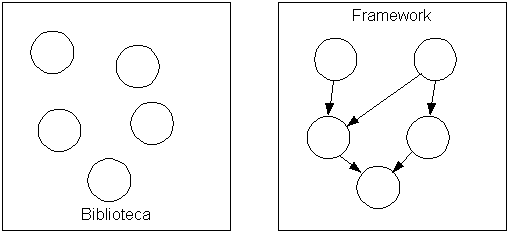
\includegraphics[width=1\textwidth]
	{Figures/biblioteca_vs_framework}
	\label{fig:biblioteca_vs_framework}
	\source{Suavé, 2001.}
\end{figure}

O ROS (Robot Operating System) é um exemplo de framework. Ele é uma plataforma de software de código aberto, desenvolvido em 2007, projetado para suportar uma nova geração de robôs. A comunidade ROS desenvolveu o framework para várias plataformas, disponibilizando-os assim para diferentes Sistemas Operacionais (SOs), como Windows, Linux e Mac OS. O ROS é um conjunto de ferramentas que gerencia de forma eficiente  a mediação entre o SO e demais aplicações, possui uma estrutura flexível permitindo a criação de software de robôs. Detém uma coleção de bibliotecas e convenções com objetivo de simplificar tarefas complexas e criar estruturas mais robustas em uma ampla gama de plataformas robóticas. Pode-se afirmar que o ROS representa uma coleção muito útil de softwares voltados exatamente para ajudar na percepção, controle e modelagem dos dispositivos de hardware que serão lidos, fornecendo serviços que são esperados de um SO, incluindo a abstração de hardware em baixo nível, o que permite a leitura e o controle do mesmo, passagem de mensagens entre processos e gerenciamento de pacotes [Quigley et al. 2009]. O ROS também disponibiliza ferramentas de aplicação de robótica nas áreas de navegação, simulação, visão, percepção e controle, sendo exemplo as bibliotecas de processamento de imagem (opencv, pcl) e simuladores (stage, gazebo).

Por ser uma plataforma com código aberto o ROS possui uma ampla documentação, bem detalhada, em sua maioria na língua inglesa. Na página da comunidade ROS, existe um extenso material de apoio, oferecendo suporte a compartilhamento de códigos fonte e experiências realizadas com o framework. A comunidade do ROS permite que o usuário faça parte dela, mediante a um cadastro pessoal no site. Dessa forma, o usuário pode deixar eventuais perguntas e/ou dúvidas que poderão ajudá-lo a solucionar algum problema.

O framework ROS foi projetado para atender a um conjunto específico de desafios encontrados durante o desenvolvimento de robôs. O ROS é muito mais do que apenas um serviço oferecido a robôs móveis e de manipulação [Alexander et al. 2012].

O ROS possui uma estrutura distribuída de processos, a qual apoia a reutilização de código em robótica. Suas bibliotecas possuem funcionalidade para diversas linguagens de de programação, foi projetado com um idioma neutro, suportando C, C++, Python, LISP e Octave, apesar de que C++ e Python são as duas linguagens principais e com maior número de pacotes disponíveis.

A comunicação do ROS é baseada em eventos, utiliza processos para publicar/subscrever nós a tópicos. Conceitualiza-se que os nós publicam e subscrevem os tópicos, permitindo assim uma comunicação entre nós, onde recebem mensagens, apenas os que estiverem subscritos ao tópico.

A Figura \ref{fig:estrutura_comunicacao_ros} demonstra uma simples publicação e subscrição de dois nós a um tópico. Desta forma sempre que o nó publicar novas mensagens os nós que estejam subscritos ao tópico irão receber a informação.

\begin{figure}[H]
	\centering
	\caption{Estrutura de comunicação.}
	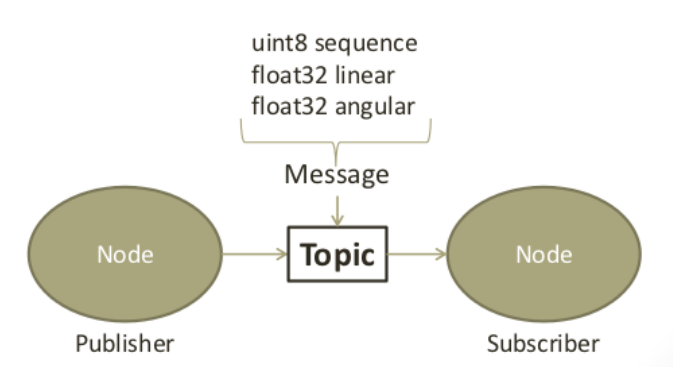
\includegraphics[width=1\textwidth]
	{Figures/estrutura_comunicacao_ros}
	\label{fig:estrutura_comunicacao_ros}
	\source{Baptista, 2013.}
\end{figure}

Os nós correspondem à execução de um programa e são criados no sistema, geralmente, via console e sempre com o servidor mestre ROS (roscore) iniciado. O servidor roscore é responsável por inicializar várias dependências, bibliotecas do ROS e o sistema de comunicação entre nós.

%--------- NEW SECTION ----------------------
\section{Estudo do Estado da Arte}
\label{sec:sota}

\subsection{GreenGiant}
\hspace{0.5cm} A Green Giant é uma desenvolvedora de múltiplas plataformas de robótica, especializada em eletrônica embarcada, tendo como seu carro-chefe o \textit{micromouse}. Seu modelo mais recente, 2016 - 2017, é voltado para alto desempenho em competições, alcançando a posição de quarto lugar durante a APEC \textit{Applied Power Electronics Conference} de 2016.

\begin{figure}[H]
	\centering
	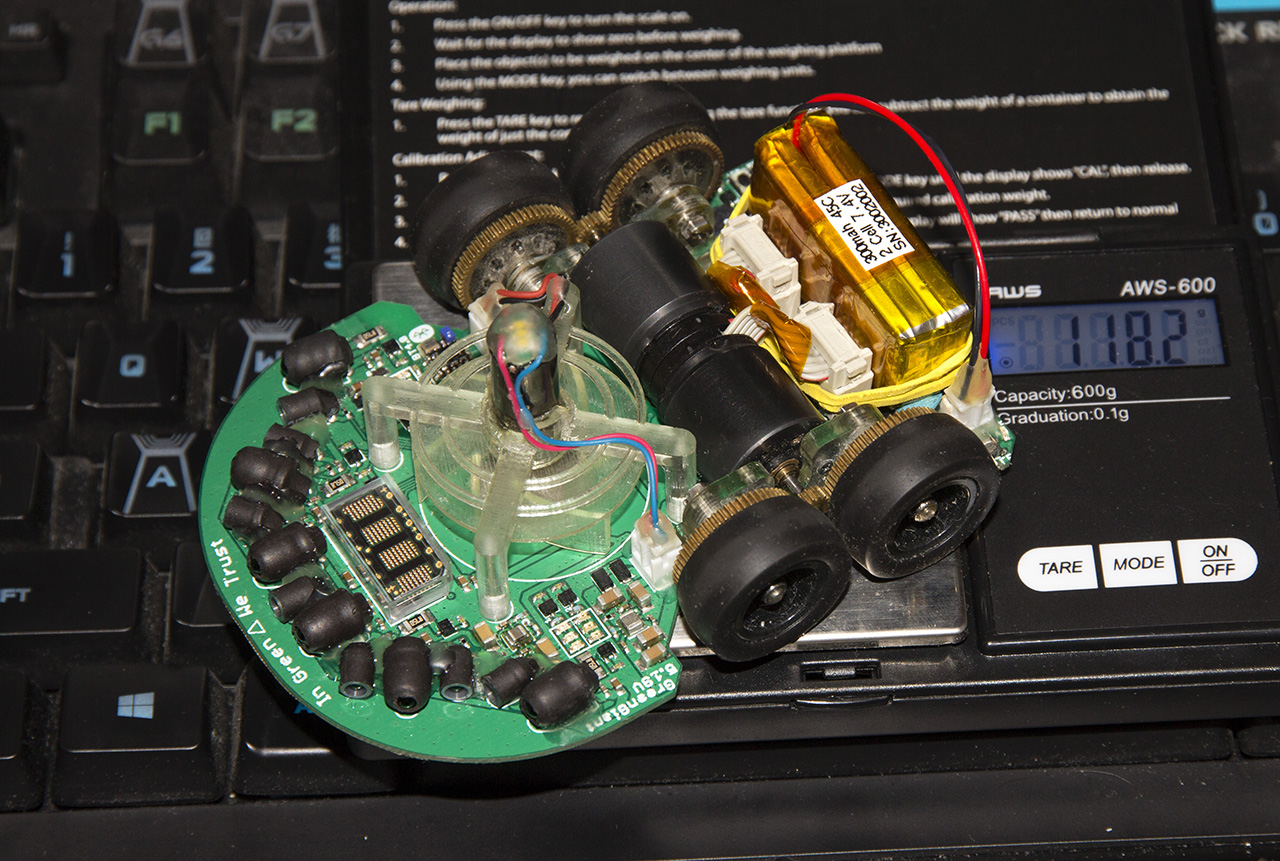
\includegraphics[width=0.7\textwidth]
	{Figures/GreenGiant_model.jpg}
	\caption{\label{fig:Green_Giant_model} Green Giant. }
	\end{figure}

\hspace{0.5cm}Sua interface de usuário possui \textit{Dot Matrix Display}, sinalizadores led, butões, buzzer, além de possuir um sistema de comunicação Bluetooth 4.0. Ademais, o modelo usa um sistema de ventoinhas de sucção para aumentar o nível de aderência das rodas, permitindo alcançar maiores velocidades sem derrapar.

\begin{table}[H]
	\centering
	\begin{tabular}{|l|l|}
		\hline
		\multicolumn{2}{|l|}{\textbf{Green Giant 5.19V}} \\ \hline
		Fabricante & Green Ye \\ \hline
		Ano & 2017 \\ \hline
		Linguagem de Programação & C/C++ \\ \hline
		Sensores & IR, MPU, IE \\ \hline
		Controlador & STM32 \\ \hline
		Simulador & - \\ \hline
		Bateria & LiPo 300mAh (7,4V) \\ \hline
		Rodas & 3D printed mount\&wheel + mini-z tyres \\ \hline
		Motor & DC-Motor 6.540RPM 0,21N.m (6V) \\ \hline
		User Interface & DMD 5x7, LEDs, Botão, Bluetooth \\ \hline
		Outros & sistema de ventoinhas de sucção \\ \hline
	\end{tabular}
	\caption{{\label{tab:Green_Giant}Green Giant}}
\end{table}


\textbf{Pontos Positivos:}
\begin{itemize}
	\item Produto de alto desempenho em competições;
	\item Sistema de ventoinhas de sucção.
\end{itemize}


\textbf{Pontos Negativos:}
\begin{itemize}
	\item Não possui suporte à simulação;
	\item Projeto pouco documentado;
	\item Não possui guia do usuário;
	\item Não possui suporte nativo para ambiente ROS.
\end{itemize}


\subsection{WPISmartMouse}
\hspace{0.5cm} A organização estudantil, WPI CollabLab, compartilham um espaço de laboratório entre seus membros para projetos com viez colaborativo a sociedade. Nesse espaço desenvolveu-se o Smartmouse, projeto \textit{micromouse} voltado para a competição Micromouse \textit{Brown IEEE Robotic  Olympiad}. O projeto também se extendeu para o desenvolvimento de um ambiente de simulação apartir dos projetos Gazebo e Ignition, não possuindo entretanto suporte para ROS.

\begin{figure}[H]
	\centering
	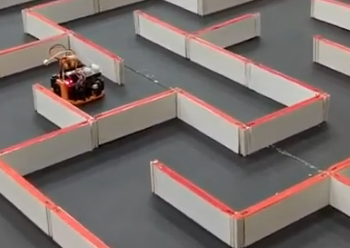
\includegraphics[width=0.7\textwidth]
	{Figures/WPISmartMouse_model.png}
	\caption{\label{fig:WPISmartMouse_model} WPISmartMouse}
\end{figure}

\begin{table}[H]
	\centering
	\begin{tabular}{|l|l|}
		\hline
		\multicolumn{2}{|l|}{\textbf{Smartmouse}} \\ \hline
		Fabricante & WPI CollabLab \\ \hline
		Ano & 2018 \\ \hline
		Linguagem de Programação & Arduino/C, Python, BASCOM \\ \hline
		Sensores & IR, Magnetic Encoder \\ \hline
		Controlador & Teensy 3.6 \\ \hline
		Simulador & Gazebo \\ \hline
		Bateria & LiPo 1500mAh (7,4V) \\ \hline
		Rodas & Solarbotics RW2i Wheel \\ \hline
		Motor & DC-Motor 650RPM 2,35Nm(6V) \\ \hline
		User Interface & LEDs \\ \hline
		Outros & documentação no git \\ \hline
	\end{tabular}
	\caption{{\label{tab:Smartmouse}Smartmouse}}
\end{table}

\textbf{Pontos Positivos:}
\begin{itemize}
	\item Provê ambiente de simulação;
	\item Documentação disponível no github;
	\item Possui portabilidade para mais de uma linguagem de programação.
\end{itemize}

\textbf{Pontos Negativos:}
\begin{itemize}
	\item Não possui suporte nativo para ambiente ROS;
	\item Pouca variedade de sensores;
	\item Não possui guia do usuário;
	\item Poucos recursos na interface com o usuário.
\end{itemize}


\subsection{Kumamoto National College}
\hspace{0.5cm} O Instituto Nacional de Tecnologia de Kumamoto, \textit{Kumamoto National College}, apresentou no ano de 2008 um projeto de desenvolvimento de ferramentas educacionais voltada para integração de sistemas e suas implementações. O projeto é direcionado aos seus estudantes do 5º ano de engenharia, através da produção de um \textit{micromouse} para a competição do ramo de \textit{Kyushu}.

\begin{figure}[H]
	\centering
	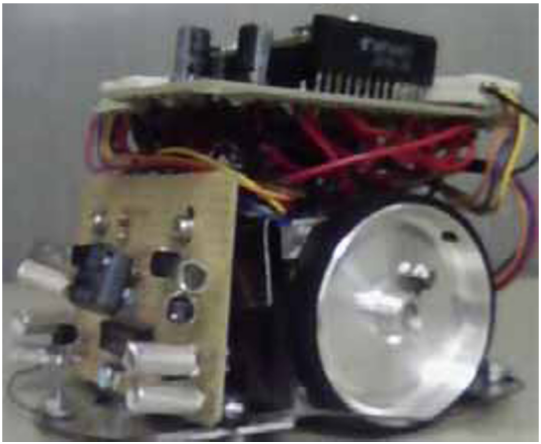
\includegraphics[width=0.7\textwidth]
	{Figures/Kumamoto_model.png}
	\caption{\label{fig:Kumamoto_model} Kumamoto.}
	\end{figure}

\hspace{0.5cm} O hardware do robô foi bastante simplificado, visando facilitar o desenvolvimento pelos estudantes ainda não familiarizados com a robótica e eletrônica, além de buscar reduzir os custos de produção do robô. Como ferramenta educativa, o projeto conseguiu que seus estudantes produzissem o \textit{micromouse} em um semestre de atividades. Contudo, conceitos da robótica (ex: robótica móvel, fusão de sensores, visão, navegação) não foram trabalhados ou não foram citados no artigo gerado a partir do projeto.


\begin{table}[H]
	\centering
	\begin{tabular}{|l|l|}
		\hline
		\multicolumn{2}{|l|}{\textbf{Kumamoto National College}} \\ \hline
		Fabricante & Kiyoteru Hayama and Tsutomu Matsumoto \\ \hline
		Ano & 2008 \\ \hline
		Linguagem & C \\ \hline
		Sensores & IR \\ \hline
		Controlador & H8Tiny-3664 \\ \hline
		Simulador & - \\ \hline
		Bateria & LiPo 900mAh (7,4V) \\ \hline
		Rodas & wheels, tires \\ \hline
		Motor & Step Motor 0,78Nm (5,6V) \\ \hline
		User Interface & LEDs \\ \hline
		Outros & Documentação em artigo \\ \hline
	\end{tabular}
	\caption{\label{tab:Kumamoto} Kumamoto}
\end{table}



\textbf{Pontos Positivos:}
\begin{itemize}
	\item Projeto com fins educacionais;
	\item Fácil desenvolvimento.
\end{itemize}

\textbf{Pontos Negativos:}
\begin{itemize}
	\item Não possui suporte nativo para ambiente ROS;
	\item Pouca variedade de sensores;
	\item Não possui guia para usuário;
	\item Poucos recursos na interface com o usuário;
	\item Não possui nenhum ambiente de simulação.
\end{itemize}


\subsection{WolfieMouse}
\hspace{0.5cm} O WolfieMouse é um projeto de robótica que desenvolveu um \textit{micromouse} para competir na \textit{2018 Region 1 Robotics Competition}.

\begin{figure}[H]
	\centering
	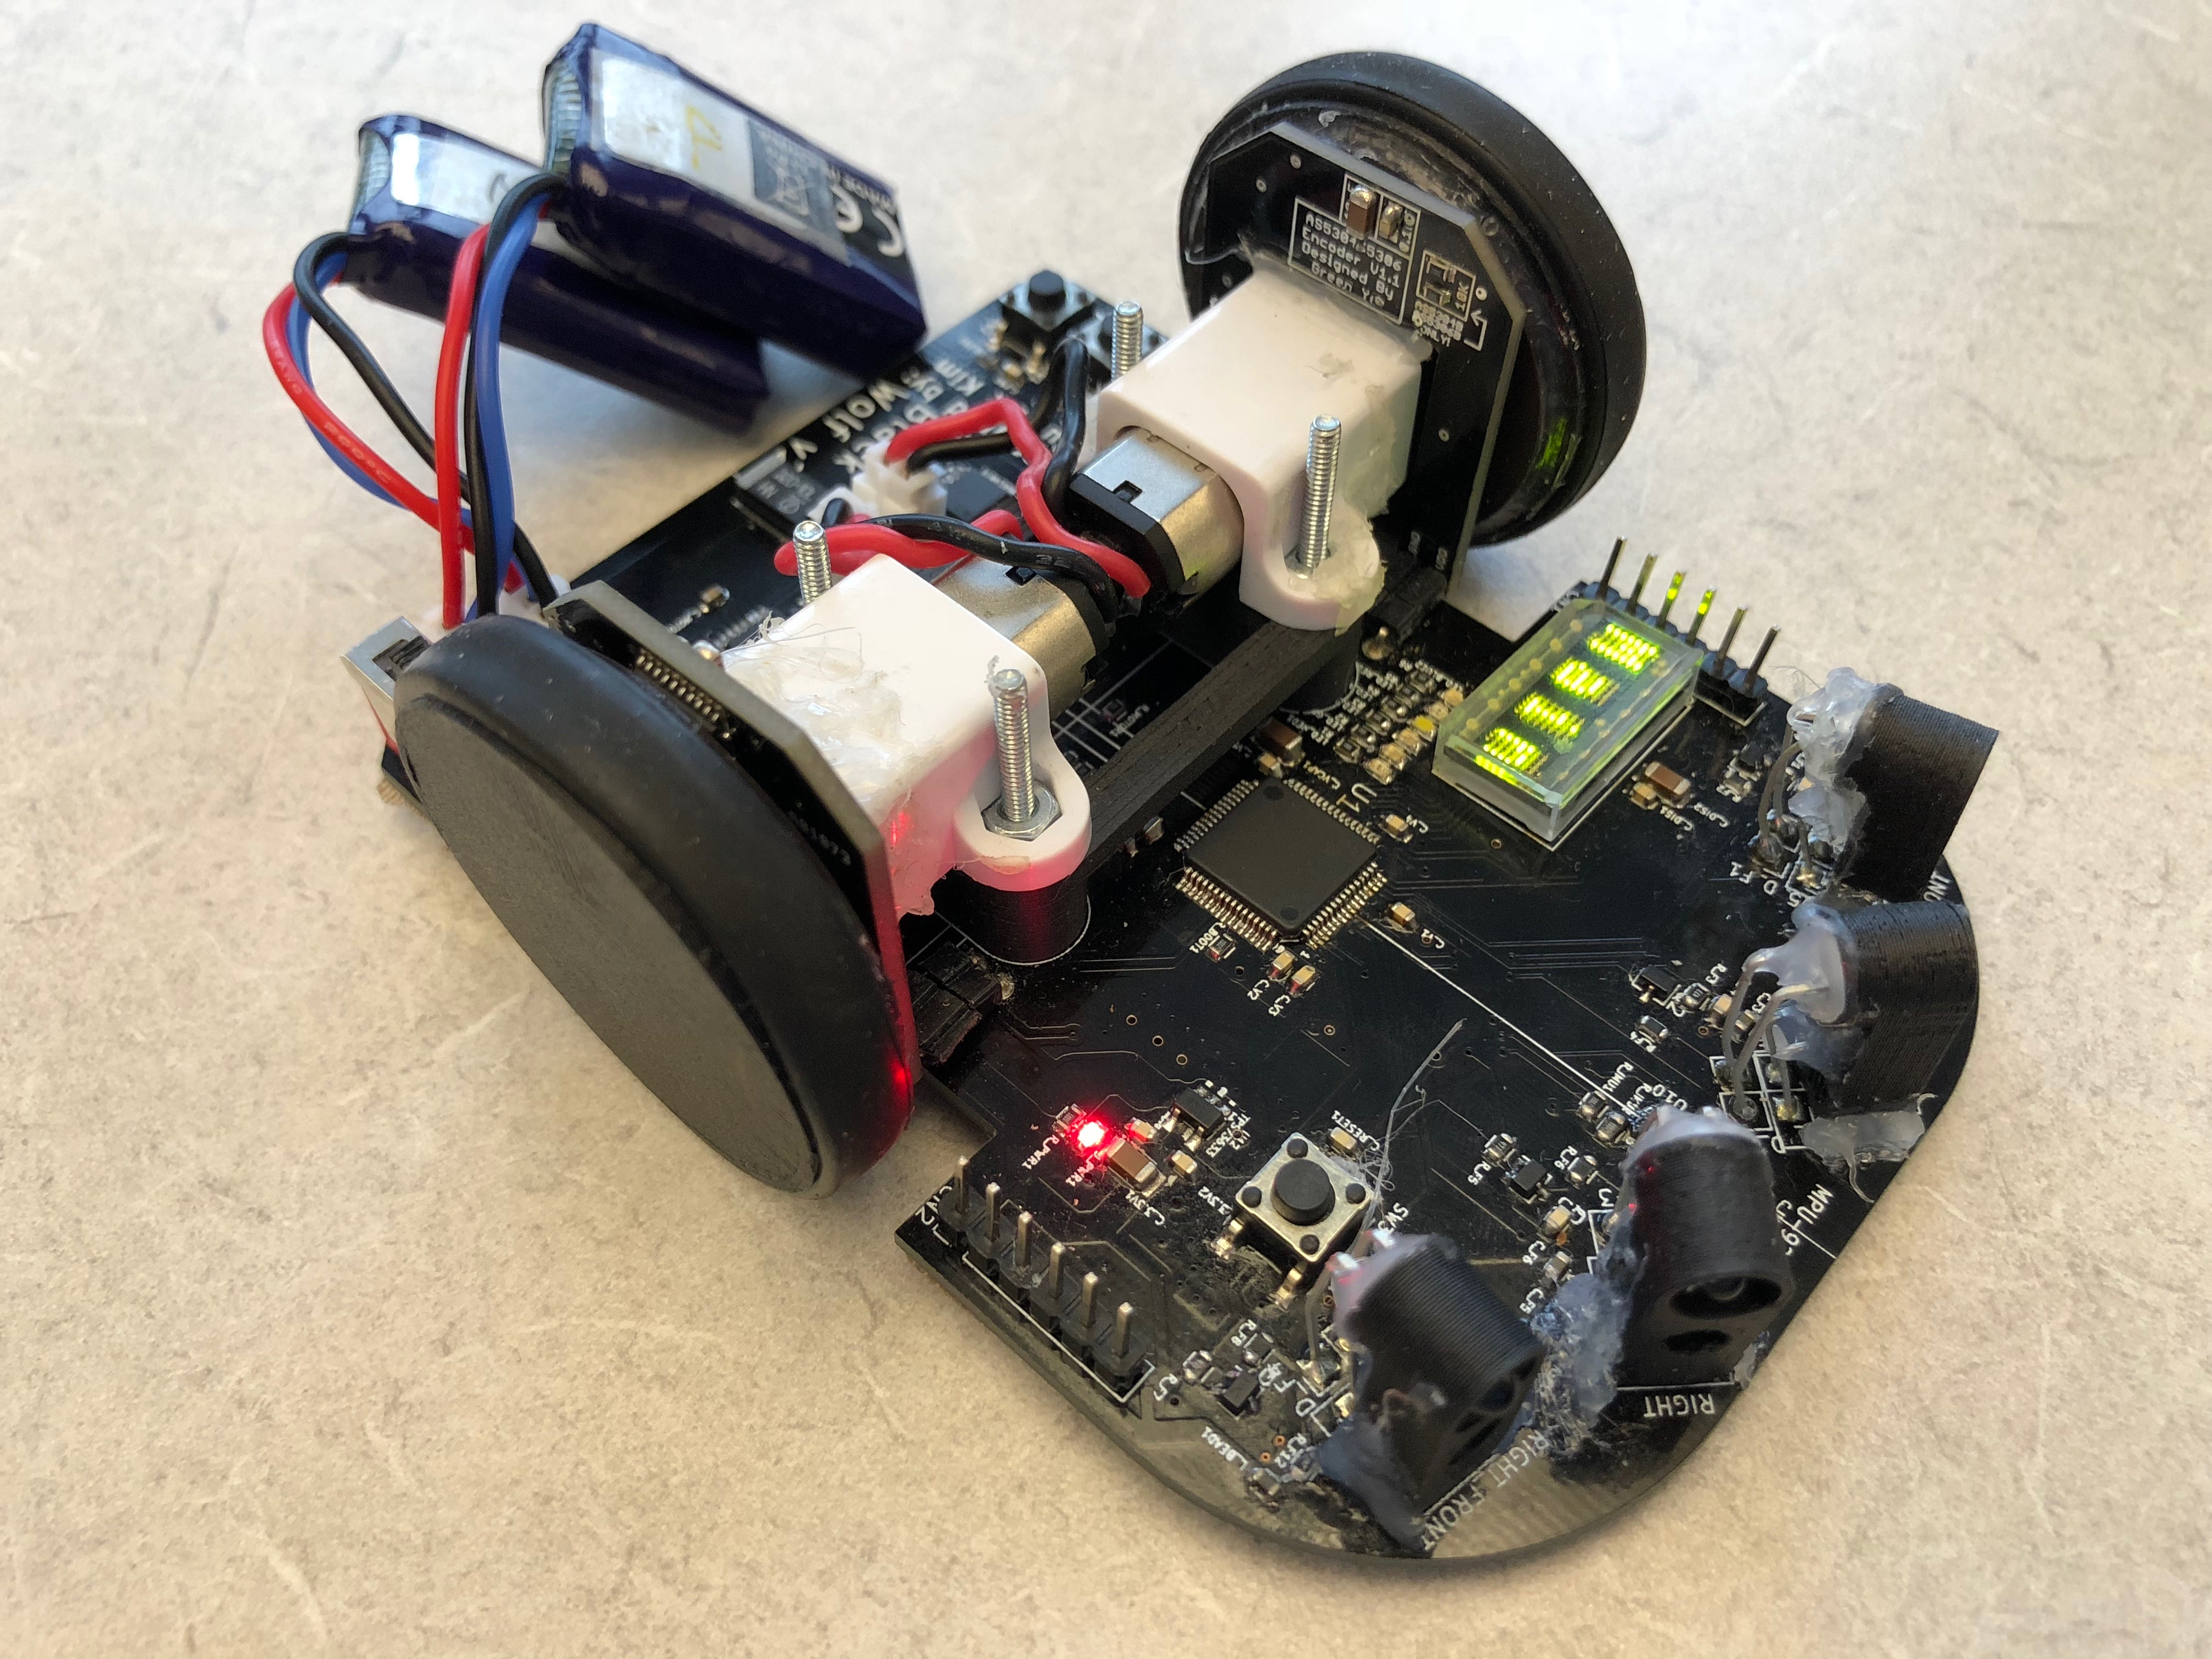
\includegraphics[width=0.7\textwidth]
	{Figures/WolfieMouse_model.jpg}
	\caption{\label{fig:WolfieMouse_model} WolfieMouse.}
\end{figure}

\hspace{0.5cm} Além da plataforma robótica, que conta com hardwares programados em baixo nível, para melhor otimização de seus controles, a equipe também realizou um ambiente de simulação baseado em C++ emulado no terminal do computador. Toda documentação foi disponibilizada em um repositório git, que também possui tutoriais para o desenvolvimento do robô.

\begin{table}[H]
	\centering
	\begin{tabular}{|l|l|}
		\hline
		\multicolumn{2}{|l|}{\textbf{WolfieMouse}} \\ \hline
		Fabricante & Bryant Gonzaga, Bum Kim, Hyun Choi \\ \hline
		Ano & 2018 \\ \hline
		Linguagem & C++, C, ARM Assembly, Python \\ \hline
		Sensores & MPU, ToF, Magnetic Encoder \\ \hline
		Controlador & STM32 \\ \hline
		Simulador & Terminal-based \\ \hline
		Bateria & * \\ \hline
		Rodas & * \\ \hline
		Motor & DC-Motor \\ \hline
		User Interface & DMD 5x7, botões \\ \hline
		Outros & documentação e tutoriais no git \\ \hline
	\end{tabular}
	\caption{\label{tab:WolfieMouse}WolfieMouse}
\end{table}

\textbf{Pontos Positivos:}
\begin{itemize}
	\item Projeto bem documentado;
	\item Possui tutoriais;
	\item Possui ambiente de simulação.
\end{itemize}

\textbf{Pontos Negativos:}
\begin{itemize}
	\item Não possui suporte nativo para ambiente ROS;
	\item Pouco foco em finalidades educativas com o produto;
	\item Não possui guia para usuário;
	\item Poucos recursos na interface com o usuário.
\end{itemize}

\subsection{Raspberry Pi Mouse V2}
\hspace{0.5cm}A RT Corporation Micromouse é uma desenvolvedora japonesa de plataformas robóticas voltada para aplicações  voltadas de pesquisas à hobistas. Um de seus segmentos é voltado para \textit{micromouse}, fortemente representado pelo seu produto Raspberry Pi Mouse V2, citado em "Learning ROS robot programming with Raspberry Pi" (Nikkei BP, June 2018).

\begin{figure}[H]
	\centering
	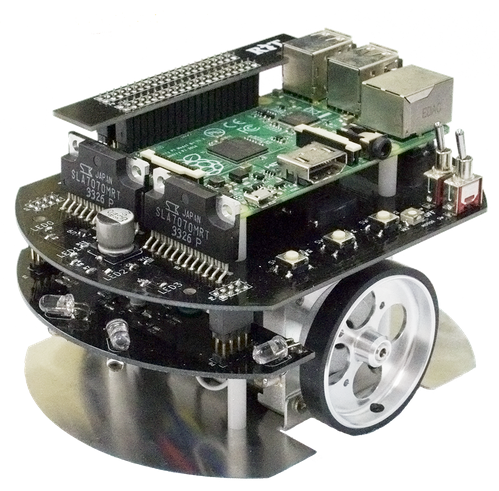
\includegraphics[width=0.7\textwidth]
	{Figures/RaspiMouse_model.png}
	\caption{\label{fig:RaspiMouse_model} RaspiMouse.}
\end{figure}
 O modelo citado, é um robô de plataforma baseado em \textit{micromouse} que utiliza uma Raspberry Pi como sua placa principal. Dessa forma o robô pode ser controlado pelos principais middleware de robótica (ROS/RTM), possuindo inclusive pacotes publicados na wiki do ROS voltados para navegação e simulação do \textit{micromouse};

\begin{table}[]
	\centering
	\begin{tabular}{|l|l|}
		\hline
		\multicolumn{2}{|l|}{\textbf{Raspberry Pi Mouse V2}} \\ \hline
		Fabricante & RT Corporation \\ \hline
		Ano & 2016 \\ \hline
		Linguagem & Python, Shell \\ \hline
		Sensores & IR \\ \hline
		Controlador & RaspberryPi3 \\ \hline
		Simulador & Gazebo \\ \hline
		Bateria & LiPo 1000mAh (7,4V) \\ \hline
		Rodas & wheels, tires \\ \hline
		Motor & Step-Motor 400step/rev (4 fases) \\ \hline
		User Interface & Terminal, LEDs, Botão, Buzzer \\ \hline
		Outros & documentação no git, mas em japonês \\ \hline
	\end{tabular}
	\caption{\label{tab:RaspiMouse} RaspiMouse}
\end{table}

\textbf{Pontos Positivos:}
\begin{itemize}
	\item Projeto bem documentado;
	\item Disponível no Gitub;
	\item Possui tutoriais;
	\item Possui ambiente de simulação;
	\item Suporte aos principais middleware de robótica (ROS/RTM);
	\item Possui pacotes do ROS para seu controle;
	\item Plataforma é expansível.
\end{itemize}

\textbf{Pontos Negativos:}
\begin{itemize}
	\item Toda documentação do produto está em japonês;
	\item O robô é pouco compacto.
\end{itemize}

\subsection{Matriz de Comparação}

\begin{table}[H]
	\centering
	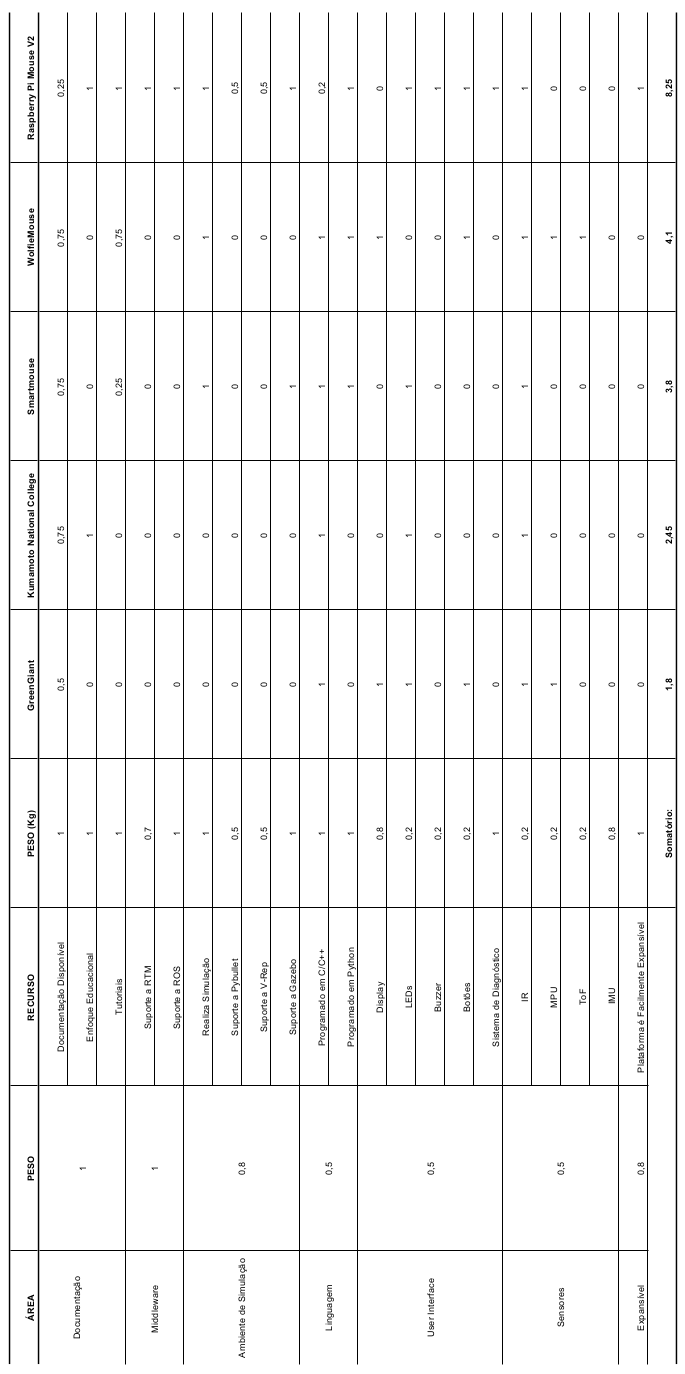
\includegraphics[width=110mm]
	{Figures/MatrizComp_v.png}
	\caption{\label{tab:MatrizComp} Matriz de Comparação.}
\end{table}